% % % % % % % % % % % % % % % % % % % % % % % % % % % % % % % % % % % % % % % % 
% LaTeX4EI Template for Cheat Sheets                                Version 1.0
%					
% Authors: Emanuel Regnath, Martin Zellner
% Contact: info@latex4ei.de
% Encode: UTF-8, tabwidth = 4, newline = LF	
% % % % % % % % % % % % % % % % % % % % % % % % % % % % % % % % % % % % % % % % 


% ======================================================================
% Document Settings
% ======================================================================

% possible options: color/nocolor, english/german, threecolumn
% defaults: color, english
\documentclass[german]{latex4ei/latex4ei_sheet}

% set document information
\title{Mathematik \\ Cheat Sheet}
\author{Raoul Duke}					% optional, delete if unchanged
\myemail{0x4723@gmail.com}			% optional, delete if unchanged
\mywebsite{www.github.com/doppelplus/}			% optional, delete if unchanged


% ======================================================================
% Define MathOperator
% ======================================================================

\DeclareMathOperator{\arcsec}{arcsec}
\DeclareMathOperator{\arccot}{arccot}
\DeclareMathOperator{\arccsc}{arccsc}
\DeclareMathOperator{\arcsinh}{asinh}
\DeclareMathOperator{\arccoth}{acoth}
\DeclareMathOperator{\arctanh}{atanh}
\DeclareMathOperator{\arccosh}{acosh}

% ======================================================================
% Begin
% ======================================================================
\begin{document}


% Title
% ----------------------------------------------------------------------
\maketitle   % requires ./img/Logo.pdf

% Tipps und Tricks
% ----------------------------------------------------------------------
\section{Allgemeines}

\begin{sectionbox}
\subsection{Zahlenmengen}\label{zahlenmengen}

\begin{itemize}
\item
  $\mathbb{N}$ = natürliche Zahlen = \{1, 2, 3, \ldots{}\}
\item
  $\mathbb{Z}$ = ganze Zahlen = \{\ldots{}, -1, 0, 1, 2, \ldots{}\}
\item
  $\mathbb{Q}$ = rationale Zahlen, z.b. \(\frac{p}{q}\) (p, q \(\in \mathbb{Z}\), q \(\neq\) 0)
\item
  $\mathbb{R}$ = reelle Zahlen, „alle Zahlen``, z.b. \(\pi\)
\item
  $\mathbb{C}$ = komplexe Zahlen = \{a + ib \textbar{} i = \(\sqrt{- 1}\), a,b \(\in \mathbb{R}\) \}
\end{itemize}

\textbf{Für Intervalle}:
Runde Klammer schließt die Grenzen aus, Eckige Klammern ein. 

\subsection{Binomialkoeffizienten}
\begin{itemize}
    \item ${n \choose j} = \frac{n!}{j!\cdot (n-j)!} \textbf{ ,für }j\leq n$
    \item  ${n \choose j} = {n \choose n-j}$
    \item  $(a+b)^n = \sum\limits_{k=0}^n {n\choose k} a^{n-k} b^k $
\end{itemize} 



\subsection{Binomische Formeln}\label{binomische-formeln}

\begin{tablebox}{ll}
1. Binomische Formel: & ${\left(a + b \right)}^{2} = {a}^{2} + 2ab + {b}^{2}$ \\
2. Binomische Formel: & ${\left(a - b \right)}^{2} = {a}^{2} - 2ab + {b}^{2}$ \\
3. Binomische Formel: & $\left(a + b \right) \left(a - b \right) = {a}^{2} - {b}^{2}$ \\
Bnomischer Lehrsatz: & ${\left( a + b \right)}^{n} = \sum _{ k = 0 }^{ n }{ { a }^{ n-k }{ b }^{ k } } $ \\
\end{tablebox}

Den Binomischen Lehrsatz kannst du auch aus dem pascalschen Dreieck entnehmen.

\subsection{Quatratische Gleichung}

\subsubsection{p-q Formel}
Grundlage ist ein Polynom: ${x}^{2} + px + q = 0$

\begin{align*}
{x}_{1/2} = - \frac{p}{2} \pm \sqrt{ {\left(\frac{p}{2}\right)}^{2} - q }
\end{align*} 

\subsubsection{Mitternachtsformel}
Grundlage ist ein Polynom: $a{x}^{2} + bx + c = 0$

\begin{align*}
{x}_{1/2} = \frac{-b \pm \sqrt{{b}^{2} - 4ac}}{2a}
\end{align*}

\subsection{Potenzrechnung}

\begin{minipage}{0.49\textwidth}
	\begin{align*}
		{a}^{n} \cdot {a}^{m} &= {a}^{n+m} \\
		{a}^{n} \cdot {b}^{n} &= {\left(a \cdot b \right)}^{n} \\
		\frac{ {a}^{n} }{ {a}^{m} } &= {a}^{n-m} \\
		\frac{{a}^{n}}{{b}^{n}} &= {\left(\cfrac{a}{b}\right)}^{n} 
	\end{align*}
\end{minipage}
\begin{minipage}{0.49\textwidth}
	\begin{align*}
		{e}^{lnx} &= x \\
		{a}^{-n} &= \frac{1}{ {a}^{n} } \\
		{-a}^{-1} &= \cfrac{-1}{a} = \cfrac{{a}^{-1}}{-1} \\
		{\left({a}^{m}\right)}^{n} &= {\left({a}^{n}\right)}^{m} = {a}^{m \cdot n}
	\end{align*}
\end{minipage}

\subsection{Bruchrechnung}\label{bruchrechnung}
\begin{tablebox}{lll}
Division & $\frac{a}{b} : \frac{c}{d} = \frac{ad}{bc}$ & Multiplizieren mit dem Kehrwert \\
Multiplikation & $\frac{a}{b} \cdot \frac{c}{d} = \frac{ac}{bd}$  \\
Kürzen & $\frac{2}{2 \cdot 3} = \frac{2}{2} \cdot \frac{1}{3} = \frac{1}{3}$ & Nur Faktoren, keine Summanden!! \\
\end{tablebox}
\textbf{Trick 17:} $\frac{x-1}{x+4} = \frac{x+4-5}{x+4} = \frac{x+4}{x+4} - \frac{5}{x+4} = 1 - \frac{5}{x+4}$

\end{sectionbox}
% Manueller Spaltenumbruch
\begin{sectionbox}

\subsection{Wurzelrechnung}

\begin{align*}
	\sqrt[n]{{a}^{m}} &= {\left({a}^{m} \right)}^{\frac{1}{n}} = {a}^{\frac{m}{n}} = {\left({a}^{\frac{1}{n}} \right)}^{m} = {\left(\sqrt[n]{a}\right)}^{m} \\
	\sqrt[m]{\sqrt[n]{a}} &= \sqrt[m]{{a}^{\frac{1}{n}}} = { \left( {a}^{\frac{1}{n}} \right) }^{ \frac{1}{m} } = {a}^{\frac{1}{m \cdot n}} = \sqrt[m \cdot n]{a} \\
	\sqrt[n]{a} \cdot \sqrt[n]{b} &= \left({a}^{\frac{1}{n}} \right) \cdot \left( {b}^{\frac{1}{n}} \right) = { \left( ab \right) }^{ \frac{1}{n} } = \sqrt[n]{ab} \\
\frac{ \sqrt[n]{a} }{ \sqrt[n]{b} } &= \frac{ {a}^{ \frac{1}{n} } }{ {b}^{ \frac{1}{n} } } = { \left( \frac{a}{b} \right) }^{\frac{1}{n}} = \sqrt[n]{ \frac{a}{b} } \text{   wenn } b  \neq 0	
\end{align*}

\subsection{Sinus \& Cosinus}
\begin{tablebox}{c|c|c|c|c}
	Bogenmaß 			& Grad 			& $\sin{x}$  & $\cos{x}$ 			& $\tan{x}$ \\ \hline
	$0 \pi$ & $0^\circ$ & $0$ & $1$ & $0$\\ \hline
	$\cfrac{1}{6} \pi$ & $30^\circ$ & $\cfrac{1}{2}$ & $\cfrac{1}{2}\sqrt{3}$ & $\cfrac{1}{\sqrt{3}}$\\ \hline
	$\cfrac{1}{4} \pi$ & $45^\circ$ & $\cfrac{1}{2}\sqrt{2}$ & $\cfrac{1}{2}\sqrt{2}$ & $1$\\ \hline
	$\cfrac{1}{3} \pi$ & $60^\circ$ & $\cfrac{1}{2}\sqrt{3}$ & $\cfrac{1}{2}$ & $\sqrt{3}$\\ \hline
	$\cfrac{1}{2} \pi$ & $90^\circ$ & $1$ & $0$ & $\pm \infty$\\ \hline
	$\cfrac{2}{3} \pi$ & $120^\circ$ & $\cfrac{1}{2}\sqrt{3}$ & $-\cfrac{1}{2}$ & $-\sqrt{3}$\\ \hline
	$\cfrac{3}{4} \pi$ & $135^\circ$ & $\cfrac{1}{2}\sqrt{2}$ & $-\cfrac{1}{2}\sqrt{2}$ & $-1$\\ \hline
	$\cfrac{5}{6} \pi$ & $150^\circ$ & $\cfrac{1}{2}$ & $-\cfrac{1}{2}\sqrt{3}$ & $-\cfrac{1}{\sqrt{3}}$\\ \hline
	$\cfrac{1}{1} \pi$ & $180^\circ$ & $0$ & $-1$ & $0$\\ \hline
	$\cfrac{7}{6} \pi$ & $210^\circ$ & $-\cfrac{1}{2}$ & $-\cfrac{1}{2}\sqrt{3}$ & $\cfrac{1}{\sqrt{3}}$\\ \hline
	$\cfrac{5}{4} \pi$ & $225^\circ$ & $-\cfrac{1}{2}\sqrt{2}$ & $-\cfrac{1}{2}\sqrt{2}$ & $1$\\ \hline
	$\cfrac{4}{3} \pi$ & $240^\circ$ & $-\cfrac{1}{2}\sqrt{3}$ & $-\cfrac{1}{2}$ & $\sqrt{3}$\\ \hline
	$\cfrac{3}{2} \pi$ & $270^\circ$ & $-1$ & $0$ & $\pm \infty$\\ \hline
	$\cfrac{5}{3} \pi$ & $300^\circ$ & $-\cfrac{1}{2}\sqrt{3}$ & $\cfrac{1}{2}$ & $-\sqrt{3}$\\ \hline
	$\cfrac{7}{4} \pi$ & $315^\circ$ & $-\cfrac{1}{2}\sqrt{2}$ & $\cfrac{1}{2}\sqrt{2}$ & $-1$\\ \hline
	$\cfrac{11}{6} \pi$ & $330^\circ$ & $-\cfrac{1}{2}$ & $\cfrac{1}{2}\sqrt{3}$ & $-\cfrac{1}{\sqrt{3}}$\\ \hline
\end{tablebox} 

$\cfrac{1}{2}\sqrt{2} \cong 0.70710678$ und $\cfrac{1}{2}\sqrt{3} \cong 0.8660254$ \\ sowie $\cfrac{1}{\sqrt{3}} \cong 0577350269$

\subsection{Ableitung trigonometrischer Funktionen}
\begin{tabular}{ccc}
	$-\cos (x)$ & $ \rightarrow$ & $\sin (x)$\\
	$\uparrow $ & 			   & $\downarrow$\\
	$-\sin (x)$	& $\leftarrow$ & $\cos (x)$\\
\end{tabular}\\
$(\tan(x))'=1+\tan^2(x) = \frac{1}{cos^2(x)}$\\
$(\cot(x))'=-\frac{1}{sin^2(x)}$\\
$(\arccos x)' = -\frac{1}{\sqrt{1-x^2}}$\\
$(\arctan x)' = \frac{1}{1+x^2}$\\
$(\arccot x)'= \frac{-1}{1+x^2}$\\


\end{sectionbox}

% Manueller Spaltenumbruch
\columnbreak

% Mengenlehre
% ----------------------------------------------------------------------
\section{Mengenlehre}

\begin{sectionbox}

\subsection{Definition}
	Ist $E$ eine Eigenschaft, die ein Element haben kann oder auch nicht, so beschreibt man die Menge der $E$ erfüllenden Elemente durch:
	
	A = $\lbrace x \vert x $ hat Eigenschaft $ E \rbrace$

\subsection{Teilmengen}
	Sind A und B Mengen, so heißt A Teilmenge oder auch Untermenge von B, wenn jedes Element von A auch Element von B ist.
	\begin{cookbox}{Merke zu Teilmengen}
		\item Jede Menge A ist Teilmenge von sich selbst, das heißt $A \subset A$
		\item Jede Menge A hat die leere Menge als Teilmenge, das heißt: $\emptyset \subset A$
		\item Ist $A \subseteq B$ und $B \subseteq C$, so folgt $A \subseteq C$
		\item Aus $A \subseteq B$ und $B \subseteq A$ folgt $A = B$
	\end{cookbox}


\subsection{Operationen}
	\begin{tablebox}{lll}
		$A \subseteq B$ &  & A ist Teilmenge von B \\
		$A \cup B$ & A vereinigt B & $A \cup B = \lbrace x \vert x \in A$ oder $x \in B \rbrace$ \\
		$A \cap B$ & A geschnitten B & $A \cap B = \lbrace x \vert x \in A$ und $x \in B \rbrace$ \\
		$A \setminus B$ & A ohne B & $A \setminus B = \lbrace x \vert x \in A$ und $x \notin B \rbrace$ \\
		$\mathcal{P}(A)$ & Potenzmenge A & Potenzmenge der Menge A\\
		$A \in B$ & A Element von B & A ist ein Element von B\\
		$A \notin B$ & A kein Element von B & A ist nicht in B enthalten \\
	\end{tablebox}
	
	
\subsection{Potenzmenge}
	Die Potenzmenge ist die Menge aller Teilmengen.
	\begin{quote}
	Es sei A eine Menge. Dann versteht man unter der Potenzmenge $\mathcal{P}(A)$ der Menge A die Menge aller Teilmengen von A. Auch die Menge $\emptyset$ hat eine Teilmenge es gilt: $\mathcal{P}(\emptyset) = \lbrace \emptyset \rbrace$.
	\end{quote}
	
	Berechnet wird die Potenzmenge mit Hilfe von $2^{\vert A \vert}$ (Zwei hoch Kardinalität von A)

\subsection{Kardinalität}
	Beschreibt die Menge aller Elemente einer Menge.
	
	\begin{quote}
	Es sei A eine endliche Menge. Dann versteht man unter der Kardinalität oder auch Mächtigkeit von A die Anzahl der Elemente von A und schreibt dafür $\vert A \vert$, manchmal auch $\#A$. Hat A unendlich viele Elemente, so sagt man, A hat die Kardinalität unendlich, und schreibt $\vert A \vert = \infty$
	\end{quote}
	
	\begin{cookbox}{Beispiel}
		$M = \lbrace 1, 2\rbrace$ \\
		$P\left(M \right) = \lbrace \lbrace \rbrace, \lbrace 1 \rbrace, \lbrace 2 \rbrace, \lbrace 1, 2 \rbrace \rbrace $ \\
		Nicht jedoch $\lbrace 2,1 \rbrace$! Es gilt $\lbrace 1,2 \rbrace = \lbrace 2,1 \rbrace$.

	\end{cookbox}

\subsection{Komplement}
	Das Komplement ist die Differenz zwischen gegebener Menge und Grundmenge. 
	
\subsection{Lösungsalgorithmus}
\begin{cookbox}{Arbeitsablauf}
		\item $\setminus$ entfernen
		\item De Morgen Gesetze anwenden
		\item Assoziativ- und Distributiv- Gesetze im Wechsel mit dem Vereinfachen
	\end{cookbox}

\subsection{Vereinfachen}
	\begin{tablebox}{lll}
		$A \cup A = A$ & $A \cap \emptyset = \emptyset $ & $\overline{\overline{A}} = A$ \\
		$A \cap A = A$ & $A \cup \overline{A} = G $ & $\overline{\emptyset} = G  $ \\
		$A \cup G = G$ & $A \cap \overline{A} = \emptyset $ & $\overline{G} = \emptyset $ \\
		$A \cap G = A$ & $\overline{A \cup B} = \overline{A} \cap \overline{B} $ & $\emptyset \neq \lbrace \emptyset \rbrace $!!! \\
		$A \cup \emptyset = A $ & $\overline{A \cap B} = \overline{A} \cup \overline{B}$ & $ $ \\
	\end{tablebox} 
	
	
\end{sectionbox}
% Manueller Spaltenumbruch
\begin{sectionbox}

\subsection{Regeln}
	\begin{tablebox}{ll}
	Kommutativ & $A \cup B = B \cup A$\\
	& $A \cap B = B \cap A$ \\
	\ctrule
	Assoziativ & $A \cap \left( B \cap C \right) = \left( A \cap B \right) \cap C$ \\
	& $A \cup \left( B \cup C \right) = \left( A \cup B \right) \cup C$ \\
	\ctrule
	Distributiv & $A \cup \left( B \cap C \right) = \left( A \cup B \right) \cap \left(A \cup C \right)$ \\
	& $A \cap \left( B \cup C \right) = \left( A \cap B \right) \cup \left(A \cap C \right)$ \\
	\ctrule
	Adjunktiv & $A \cup \left( A \cap B \right) = A $ \\
	& $A \cap \left( A \cup B \right) = A$ \\
	\ctrule
	de Morganschen Regeln & $A \setminus \left( B \cap C \right) = \left( A \setminus B \right) \cup \left( A \setminus C \right)$ \\
	& $A \setminus \left( B \cup C \right) = \left( A \setminus B \right) \cap \left( A \setminus C \right)$ \\
	\ctrule
	de Morganschen Gesetz & $A \setminus B = A \cap \overline{B}$ \\
	\end{tablebox}

\subsection{Kartesisches Produkt}
Das kartesische Produkt $A\times B$ (A kreuz B) ist die Menge aller geordneten Paare $\left( a , b \right)$ mit $a \in A$ und $b \in B$


\end{sectionbox}

% Relationen
% ----------------------------------------------------------------------
\section{Relationen}

\begin{sectionbox}

\subsection{Definition}
	Eine (zweistellige) Relation $R$ ist eine Teilmenge des kartesischen Produkts zweier Mengen $A$ und $B$.

	\begin{quote}
		$R \subseteq A\times B$
	\end{quote}

\subsection{Äquivalenzrelation}
	Eine Äquivalenzrelation ist eine zweistellige Relation auf einer Ausgangsmenge $M$ mit bestimmten Eigenschaften.

	\begin{quote}
		$R \subseteq M\times M$
	\end{quote}

	\begin{cookbox}{Eigenschaften}
		\item \textbf{Reflexivität}

		Jedes Element der Ausgangsmenge $M$ steht mit sich selbst in Beziehung.

		\begin{quote}
			Für alle $a \in M$ gilt $\left( a , a \right) \in R$
		\end{quote}

	\item \textbf{Symmetrie}

	Zu jedem Paar $\left( a , b \right)$ ist auch die Umkehrung in $R$ enthalten.

	\begin{quote}
		Wenn $\left( a , b \right) \in R$, dann ist auch $\left( b , a \right) \in R$
	\end{quote}

	\item \textbf{Transitivität}

	Stehen drei Elemente verkettet in Beziehung, dann stehen sie auch direkt in Beziehung.

	\begin{quote}
		Wenn $\left( a , b \right) , \left( b , c \right) \in R$ dann ist auch $\left(a , c \right) \in R$
	\end{quote}

	\end{cookbox}

\end{sectionbox}

\newpage % Hilfestellung um die Aussagenlogik auf einer Seite zu haben.

% Aussagenlogik
% ----------------------------------------------------------------------
\section{Aussagenlogik}

\begin{sectionbox}

\subsection{Operationen}
	\begin{tablebox}{lll}
		$A \wedge B$ & A und B & Konjunktion\\
		$A \vee  B$ & A oder B & Disjunktion \\
		$A \leftrightarrow B$ & A genau dann, wenn B & Äquivalenz oder Bijunktion \\
		$A \rightarrow B$ & wenn A dann B & Implikation oder Subjunktion \\
	\end{tablebox}
	
\subsection{Regeln}
	\begin{tablebox}{ll}
	Kommutativ & $A \wedge B = B \wedge A$\\
	& $A \vee B = B \vee A$ \\
	& $A \leftrightarrow B = B \leftrightarrow A$  \\
	\ctrule
	Assoziativ & $A \wedge \left( B \wedge C \right) = \left( A \wedge B \right) \wedge C$ \\
	& $A \vee \left( B \vee C \right) = \left( A \vee B \right) \vee C$ \\
	& $A \leftrightarrow \left( B \leftrightarrow C \right) = \left( A \leftrightarrow B \right) \leftrightarrow C$ \\
	\ctrule
	Distributiv & $A \wedge \left( B \vee C \right) = \left( A \wedge B \right) \vee \left(A \wedge C \right)$ \\
	& $A \vee \left( B \wedge C \right) = \left( A \vee B \right) \wedge \left(A \vee C \right)$ \\
	& $A \rightarrow \left( B \vee C \right) = \left( A \rightarrow B \right) \vee \left(A \rightarrow C \right)$ \\
	& $A \rightarrow \left( B \wedge C \right) = \left( A \rightarrow B \right) \wedge \left(A \rightarrow C \right)$ \\
	& $\left( A \vee B \right) \rightarrow C = \left( A \rightarrow C \right) \wedge \left(B \rightarrow C \right)$ \\
	& $\left( A \wedge B \right) \rightarrow C = \left( A \rightarrow C \right) \vee \left(B \rightarrow C \right)$ \\
	\ctrule
	Adjunktiv (Absorbtion) & $A \wedge \left( A \vee B \right) = A $ \\
	& $A \vee \left( A \wedge B \right) = A$ \\
	\ctrule
	Klammerntausch & $A \rightarrow \left( B \rightarrow C \right) = \left( A \wedge B \right) \rightarrow C  $ \\
	\ctrule
	Kontraposition & $A \rightarrow B  = \neg B \rightarrow \neg A  $ \\
	\ctrule
	de Morganschen Regeln & $\neg \left( A \vee B \right) = \neg A \wedge \neg B$ \\
	& $\neg \left( A \wedge B \right) = \neg A \vee \neg B$ \\

	Umwandeln & $A \wedge B = \neg \left( A \rightarrow \neg B \right)$ \\
	& $A \vee B = \neg A \rightarrow B $ \\
	& $A \rightarrow B = \neg A \vee B$ \\
	& $A \leftrightarrow B  = \left( A \wedge B \right) \vee \left(\neg A \wedge \neg B \right)$ \\
	& $A \leftrightarrow B  = \left( \neg A \vee B \right) \wedge \left(A \vee \neg B \right)$ \\
	\ctrule
	Vereinfachen & $A \wedge \neg A = $ immer Falsch! \\
	& $A \vee \neg A = $ immer Richtig! \\
	& $A \wedge \neg A \vee B \wedge A = B \wedge A$ \\
	\end{tablebox}

\subsection{Beispiel}
	Günter fragt Anna: "Libst du Peter, oder ist es nicht so, dass du Peter oder mich liebst?", darauf Antwortet Anna "Nein". \\
	Für die Aussage Anna liebt Peter setzen wir P und für Anna liebt Günther G. Die Frage lautet somit "Gilt P, oder gilt nicht P $\wedge$ G?". Formal bedeutet das:
	\begin{quote}
		$P \vee \neg \left( P \vee G \right)$ \\
	\end{quote}
	
	Da Anna mit "Nein" Antwortet muss der ganze Block negativiert werden.
	\begin{quote}
		$\neg \left( P \vee \neg \left( P \vee G \right)\right)$ \\
	\end{quote}
	 
\subsection{Wahrheitstafeln}
\begin{minipage}{0.49\textwidth}
	\textbf{Konjunkiton} (UND)
	\begin{tablebox}{|l|l|l|}
		\hline
		$A $ & $B$ & $A \wedge B$ \\ \hline
		$0$ & $0$ & $0$ \\ \hline
		$0$ & $1$ & $0$ \\ \hline
		$1$ & $0$ & $0$ \\ \hline
		$1$ & $1$ & $1$ \\ \hline
	\end{tablebox}
\end{minipage}
\begin{minipage}{0.49\textwidth}
	\textbf{Disjunktion} (ODER)
	\begin{tablebox}{|l|l|l|}
		\hline
		$A $ & $B$ & $A \vee B$ \\ \hline
		$0$ & $0$ & $0$ \\ \hline
		$0$ & $1$ & $1$ \\ \hline
		$1$ & $0$ & $1$ \\ \hline
		$1$ & $1$ & $1$ \\ \hline
	\end{tablebox}
\end{minipage}

\end{sectionbox}
% Manueller Spaltenumbruch
\begin{sectionbox}


\begin{minipage}{0.49\textwidth}
	\textbf{Bijunktion} (ist richtig wenn beide gleich sind)
	\begin{tablebox}{|l|l|l|}
		\hline
		$A $ & $B$ & $A \leftrightarrow B$ \\ \hline
		$0$ & $0$ & $1$ \\ \hline
		$0$ & $1$ & $0$ \\ \hline
		$1$ & $0$ & $0$ \\ \hline
		$1$ & $1$ & $1$ \\ \hline
	\end{tablebox}
\end{minipage}
\begin{minipage}{0.49\textwidth}
	\textbf{Implikation} (aus A folgt B)
	\begin{tablebox}{|l|l|l|}
		\hline
		$A $ & $B$ & $A \rightarrow B$ \\ \hline
		$0$ & $0$ & $1$ \\ \hline
		$0$ & $1$ & $1$ \\ \hline
		$1$ & $0$ & $0$ \\ \hline
		$1$ & $1$ & $1$ \\ \hline
	\end{tablebox}
\end{minipage}

\begin{tablebox}{|l|l|l|l|l|l|l|}
		\hline
		$A $ & $B$ & $C$ & $A \wedge B$ & $A \vee B$ & $A \wedge B \rightarrow A \vee B$ & $G$\\ \hline
		$0$ & $0$ & $0$ & $0 $ & $0 $ & $1 $ & $0 $ \\ \hline
		$0$ & $0$ & $1$ & $0 $ & $0 $ & $1 $ & $1 $ \\ \hline
		$0$ & $1$ & $0$ & $0 $ & $1 $ & $1 $ & $0 $ \\ \hline
		$0$ & $1$ & $1$ & $0 $ & $1 $ & $1 $ & $1 $ \\ \hline
		$1$ & $0$ & $0$ & $0 $ & $1 $ & $1 $ & $0 $ \\ \hline
		$1$ & $0$ & $1$ & $0 $ & $1 $ & $1 $ & $1 $ \\ \hline
		$1$ & $1$ & $0$ & $1 $ & $1 $ & $1 $ & $0 $ \\ \hline
		$1$ & $1$ & $1$ & $1 $ & $1 $ & $1 $ & $1 $ \\ \hline
	\end{tablebox}

\end{sectionbox}


% Komplexe Zahlen
% ----------------------------------------------------------------------
\section{Komplexe Zahlen}

\begin{sectionbox}

\subsection{Notation}
\begin{minipage}{0.39\textwidth}
	\textbf{Kartesische Form}\\
	$z = a+b \cdot i$
\end{minipage}
\begin{minipage}{0.59\textwidth}
	\textbf{Trigonometrische Form / Polarform}\\
	$z =\left| z \right| \cdot \left( \cos { \varphi } + i \cdot \sin { \varphi  } \right)$
\end{minipage}

\subsection{Visualisierung}
\begin{minipage}{0.49\textwidth}
	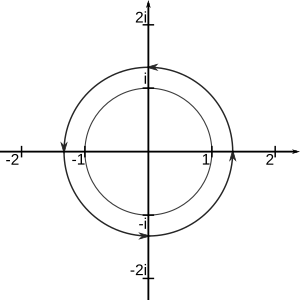
\includegraphics[width=\textwidth]{img/einheitskreis_komplexe_zahlen.png}
\end{minipage}
\begin{minipage}{0.49\textwidth}
	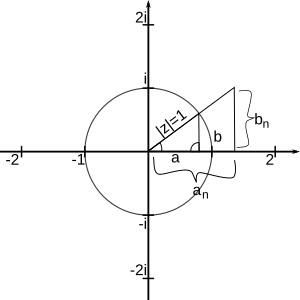
\includegraphics[width=\textwidth]{img/visualisierung_komplexe_zahlen.png}
\end{minipage}

	\begin{tablebox}{lll}
		$\vert z \vert = \sqrt{ {a}^{2} + {b}^{2} }$& $\varphi = \arctan \left( \cfrac{b}{a} \right) $ & siehe Tabelle xxx \\
		$\tan\left(\varphi\right) = \cfrac{\vert b \vert}{ \vert a \vert}$ & $\cos\left(\varphi\right) = \cfrac{a}{\vert z \vert}$  & $\sin\left(\varphi\right) = \cfrac{b}{\vert z \vert}$ \\
	\end{tablebox} 
	
	\begin{tablebox}{l|l|l}
\textbf{x,y} & \textbf{(in Grad)} & \textbf{(im Bogenmaß)} \\ \hline	
$a > 0, b \ge 0$    & $\varphi = \arctan \cfrac{b}{a} $ & $\varphi = arctan \cfrac{b}{a}$  \\
$a < 0$   & $\varphi = \arctan \cfrac{b}{a} + 180^\circ $ & $\varphi = arctan \cfrac{b}{a} + \pi $ \\
$a > 0, b \le 0 $ & $\varphi = \arctan \cfrac{b}{a} + 360^\circ $  & $\varphi = \arctan \cfrac{b}{a} + 2\pi $   \\
$a = 0, b > 0 $ & $\varphi = 90^\circ $ &   $\varphi = \cfrac{\pi}{2} $           \\
$a = 0, b < 0 $   & $\varphi = 270^\circ $     &      $\varphi = \cfrac{3}{2}\pi $        \\
$a = 0, b = 0 $   & $\varphi = 0^\circ $    &       $\varphi = 0 $       \\ 
\end{tablebox}

\subsection{Potenzen von i}

\begin{tablebox}{ll}
		$i = \sqrt{-1} $ & ${ i }^{ 4 } = 1 $ \\
		${ i }^{ 2 } = -1$ & ${ i }^{ 5 } = i$  \\
		${ i }^{ 3 } = -i$ & ${ i }^{ 6 } = -1 $...  \\
	\end{tablebox} 

\end{sectionbox}
% Manueller Spaltenumbruch
\begin{sectionbox}

\subsection{Rechenoperationen}
\begin{minipage}{0.49\textwidth}
	\textbf{Addition}
\begin{align*}
	 { z }_{ 1 } + { z }_{ 2 } &= \left(a + bi\right) + \left(c + di \right)\\
	 &= a + c + (b + d)i
	\end{align*}
\end{minipage}
\begin{minipage}{0.49\textwidth}
	\textbf{Subtraktion}
	\begin{align*}
	 { z }_{ 1 } - { z }_{ 2 } &= \left(a + bi \right) - \left(c + di \right)\\
	 &= a - c + (b - d)i
	\end{align*}
\end{minipage}

\textbf{Multiplikation}
\begin{align*}
	 { z }_{ 1 } \cdot  { z }_{ 2 } &= \left(a + bi \right) \cdot \left(c + di \right) \\
	 &= ac + adi + bci + bd { i }^{ 2 }
	\end{align*}
	\begin{align*}
	{ z }_{ 1 }\cdot { z }_{ 2 } & =\left| { z }_{ 1 } \right| \left( \cos { \left( { \varphi  }_{ 1 } \right)  } +\sin { \left( { \varphi  }_{ 1 } \right)  } i \right) \cdot \left| { z }_{ 2 } \right| \left( \cos { \left( { \varphi  }_{ 2 } \right)  } \cdot \sin { \left( { \varphi  }_{ 2 } \right)  } i \right) \\ 
	& =\left| { z }_{ 1 } \right| \cdot \left| { z }_{ 2 } \right| \left( \cos { \left( { \varphi  }_{ 1 } + { \varphi  }_{ 2 } \right)  } +\sin { \left( { \varphi  }_{ 1 } + { \varphi  }_{ 2 } \right)  } i \right)
	\end{align*}

\textbf{Division}
\begin{align*}
\frac { z_{ 1 } }{ z_{ 2 } } &=\frac { a+bi }{ c+di } \quad =\frac { \left( a+bi \right)  }{ \left( c+di \right)  } \cdot \frac { \left( c-di \right)  }{ \left( c-di \right)  } \\ 
&=\frac { ac\quad -\quad adi\quad +\quad bci\quad -\quad bd{ i }^{ 2 } }{ { c }^{ 2 }-{ \left( di \right)  }^{ 2 } } \\ 
&=\frac { ac+bd+\left( bc-ad \right) i }{ { c }^{ 2 }+{ d }^{ 2 } } \\ 
&=\frac { ac+bd }{ { c }^{ 2 }+{ d }^{ 2 } } +\frac { \left( bc-ad \right)  }{ { c }^{ 2 }+{ d }^{ 2 } }  i
\end{align*}

\textbf{Potenzierung}
\begin{align*}
{ z }^{ n } &={ \left( a+bi \right)  }^{ n } \\
&={ \left( \left| z \right| \cdot \left( \cos { \varphi  } +\sin { \varphi  } i \right)  \right)  }^{ n } \\
&={ \left| z \right|  }^{ n }\cdot \left( \cos { \left( n\cdot \varphi  \right)  } +\sin { \left( n\cdot \varphi  \right)  } i \right)
\end{align*}

\textbf{Wurzel} $\lbrace k \in \mathbb{N}  \vert k = 0$ bis $n-1 \rbrace$
\begin{align*}
\sqrt[n]{z} &= \sqrt[n]{ a+bi } \\
{ z }_{ k } &= \sqrt[n]{\vert z \vert} \cdot \left( \cos{ \left( \cfrac{ \varphi + k \cdot 360}{n} \right) } +\sin{\left( \cfrac{\varphi + k \cdot 360}{n} \right)} i \right) 
\end{align*}
Es gibt immer $n$ Ergebnisse die in ${ z }_{ k } $ für $k= 0$ bis $k= n-1$ berechnet werden.

\end{sectionbox}

% Vektoren und Matritzen
% ----------------------------------------------------------------------
\section{Vektoren und Matritzen}

\begin{sectionbox}
Matritzen vom Typ (m,1) sind Vektoren (1-Spaltig). Die Zeilen eines Vektors sind auch die Dimension des Vektors. Ein Zeilen Vektor ist eine Matritze vom Typ (1, n).

\subsection{Rechenoperationen}
\subsubsection{Skalar}
Die Addition, Subtraktion und Multiplikation von Matritzen mit einem Skalar (einer Zahl) c.
\begin{align*}
-1 \cdot A &= -A \\ 
c \cdot A &= A \cdot c = Ac = cA \\
{c}_{1} \cdot \left( {c}_{2} \cdot A \right) &= \left( {c}_{1} \cdot {c}_{2} \right) \cdot A \\\left({c}_{1} + {c}_{2} \right) \cdot A &= {c}_{1} \cdot A + {c}_{2} \cdot A \\
c \cdot \left(A + B \right) &= cA + cB 
\end{align*}

\subsubsection{Multiplikation}
\begin{itemize}
\item Zeile von Matrix A mal Spalte von Matrix B 
\item Matrix A muss so viele Spalten haben wie Matrix B Zeilen hat 
\item Nicht Kommutativ!! $A \cdot B \neq B \cdot A$
\end{itemize}

\end{sectionbox}
% Manueller Spaltenumbruch
\begin{sectionbox}

\subsubsection{Determinante}
\begin{itemize}
\item Ist $\det A \neq 0$ dann ist die Matrix invertierbar
\item Ist $\det A = 0$ dann ist die Matrix Linear abhängig
\item Schachbrettmuster (beginnend oben links mit + - + -..)
\item Entwicklung am einfachsten nach der Spalte oder Zeile mit den meisten 0er.
\end{itemize}

\begin{align*}
A &= \begin{pmatrix} 0 & 1 & 3 \\ 4 & 2 & 0 \\ 0 & 1 & 5 \end{pmatrix} \\
det A &= -4 \cdot \begin{vmatrix} 1 & 3 \\ 1 & 5 \end{vmatrix} \\
&= -4 \cdot \left(1*5 - 1*3\right) = -8
\end{align*}

\subsection{Inverse Matrix}
Invertierbar sind nur Matritzen des Typ (n, n) also quadratische Matritzen.
Eine Matrix ist dann Invertierbar wenn die Determinante $ \neq $ 0 ergibt. 
\begin{tablebox}{ll}
${A}^{-1} \cdot A = I$ & ${\left( A \cdot B \right)}^{-1} = {B}^{-1} \cdot {A}^{-1}$ \\
$A \cdot {A}^{-1} = I$ & $I \cdot A = A $ \\
$I \cdot {A}^{-1} = {A}^{-1}$ &  \\
\end{tablebox}

\end{sectionbox}


% Vektoren
% ----------------------------------------------------------------------
\section{Vektoren}

\begin{sectionbox}

\subsection{Vektor Aufstellen}

\begin{minipage}{0.49\textwidth}
\begin{align*}
 A &= \begin{pmatrix} {a}_{1} & {a}_{2} & {a}_{3} \end{pmatrix}  \\ 
 B &= \begin{pmatrix} {b}_{1} & {b}_{2} & {b}_{3} \end{pmatrix}
\end{align*}

\end{minipage}
\begin{minipage}{0.49\textwidth}
\begin{align*}
\overrightarrow{AB} = \begin{pmatrix}
{b}_{1} - {a}_{1} \\
{b}_{2} - {a}_{2} \\
{b}_{3} - {a}_{3} \\
\end{pmatrix}
\end{align*}
\end{minipage}

\subsection{Rechenoperation}
\begin{tablebox}{ll}
Addition & $ \overrightarrow{a} + \overrightarrow{b} = \begin{pmatrix} {a}_{1} \\ {a}_{2} \end{pmatrix} + \begin{pmatrix} {b}_{1} \\ {b}_{2}\end{pmatrix} = \begin{pmatrix} {a}_{1} + {b}_{1} \\ {a}_{2} + {b}_{2} \end{pmatrix} $ \\
Multiplikation & $ \overrightarrow{a} = c \cdot \begin{pmatrix} {b}_{1} \\ {b}_{2} \end{pmatrix} = \begin{pmatrix} c {b}_{1} \\ c {b}_{2} \end{pmatrix} $ \\
Betrag & $ \vert \overrightarrow{a} \vert = \sqrt{{{a}_{1}}^{2} + {{a}_{1}}^{2} } $ \\
Skalarpordukt & $\overrightarrow{a} \ast \overrightarrow{b} = {a}_{1}{b}_{1} + {a}_{2}{b}_{2} + {a}_{3}{b}_{3} $ \\
Kreuzprodukt & $\overrightarrow{a} \times \overrightarrow{b} = \overrightarrow{n} = \begin{pmatrix}
{a}_{2}{b}_{3} - {a}_{3}{b}_{2} \\
{a}_{3}{b}_{1} - {a}_{1}{b}_{3} \\
{a}_{1}{b}_{2} - {a}_{2}{b}_{1} \\
\end{pmatrix} $ \\
\end{tablebox}
Ist das Skalarprodukt = 0 dann sind die Vektoren orthogonal (senkrecht) zueinander!


\end{sectionbox}


\columnbreak % Manueller Zeilenumbruch

% Geraden und Ebenen
% ----------------------------------------------------------------------
\section{Geraden und Ebenen}

\begin{sectionbox}
\subsection{Schnittpunkte}
\begin{minipage}{0.49\textwidth}
\textbf{Gerade}
Den Schnittpunkt von zwei geraden erhält man indem man die beiden Geradengleichungen gleich setzt.
\end{minipage}
\begin{minipage}{0.49\textwidth}
\textbf{Ebene}
Bei Einer Ebene funktioniert die Berechnung des Schnittpunktes analog zu dem einer Geraden.
\end{minipage}

\subsection{Winkel}
\begin{minipage}{0.49\textwidth}
\textbf{Gerade und Gerade}
\begin{align*}
\cos \alpha = \left| \frac{\xrightarrow{a} \cdot \xrightarrow{b} }{\vert \xrightarrow{a} \vert \cdot \vert \xrightarrow{b} \vert} \right|
\end{align*}
\end{minipage}
\begin{minipage}{0.49\textwidth}
\textbf{Gerade und Ebene}
\begin{align*}
\cos \alpha = \left| \frac{\xrightarrow{a} \cdot \xrightarrow{b} }{\vert \xrightarrow{a} \vert \cdot \vert \xrightarrow{b} \vert} \right|
\end{align*}
\end{minipage}

\subsection{Formen}
\subsubsection{Geraden}
Allgemeine Form: 
\begin{align*}
\overrightarrow{x} = \overrightarrow{p} + t \cdot \overrightarrow{u}
\end{align*} 
$\overrightarrow{p}$ = Stützvektor und $\overrightarrow{u}$ = Richtungsvektor.

\subsubsection{Ebenen}
\begin{tablebox}{ll}
Parameterform & 
$E:\overrightarrow{x} = \overrightarrow{p} + t \cdot \overrightarrow{u} + s \cdot \overrightarrow{v} $ \\
Normalform & $\overrightarrow{n} \cdot \left( \overrightarrow{x} - \overrightarrow{p} \right) = 0 $\\
\end{tablebox}
$\overrightarrow{p}$ = Stützvektor und $\overrightarrow{u}$,$\overrightarrow{v}$ = Spannvektor

\textbf{Umformen:}
\begin{enumerate}
	\item Parameter $\rightarrow$ Normalform
	\item $\overrightarrow{n} = \overrightarrow{u} \times \overrightarrow{v}$ (Kreuzprodukt der Richtungsvektoren 
	\item $\overrightarrow{n} \cdot \left( \overrightarrow{x} - \overrightarrow{p} \right) = 0 $
	\item Koordinatenform aufstellen \\
	$\overrightarrow{n} \cdot \overrightarrow{x} = \overrightarrow{n} \cdot \overrightarrow{p}$
	(Normalform aus multipliziert)
\end{enumerate}


\end{sectionbox}


% Grenzwerte
% ----------------------------------------------------------------------
\section{Grenzwerte}

\begin{sectionbox}
Der Grenzwert oder Limes einer Folge ist eine Zahl, der die Folge beliebig nah kommt. Eine Folge ist \textbf{konvergent} wenn sie solch einen Wert besitzt, ansonsten \textbf{divergent}

\subsection{Berechnung}
Bei $n \rightarrow \infty$ teilt man durch die variable mit der höchsten Potenz, das Ergebnis ist dann der Grenzwert.
\begin{align*}
&\lim\limits_{n \rightarrow \infty}{\frac{2{n}^{2} -1}{{n}^{2} + 1}} = \lim\limits_{n \rightarrow \infty}{ \frac{ 2 - \frac{1}{ {n}^{2} } }{1 + \frac{ 1 }{ {n}^{2} }} } =\frac{ \lim\limits_{n \rightarrow \infty}{ 2{n}^{2} -1 } }{ \lim\limits_{n \rightarrow \infty}{ {n}^{2} + 1} } = \frac{2}{1} = 2
\end{align*}

\textbf{Ergebnisse}
\begin{tablebox}{llll}
$\frac{1}{1} = 1 $ & $\frac{1}{0} = \infty $ & $\frac{0}{1} = 0 $ & $\frac{1}{17} = \frac{1}{17}$ \\
\end{tablebox}

\textbf{Vorsicht} bei $\lim\limits_{n \rightarrow a}$, also Limes gegen eine Zahl a. Zunächst setzt man die Zahl a ein und prüft das Ergebnis. Es darf nicht $\frac{0}{0}$ raus kommen. Es wird sich im Zähler und/oder Nenner ein $n - a$ befinden. Die Folge muss dann in Linearfaktoren zerlegt werden und danach die 3 eingesetzt werden. 
\begin{align*}
&\lim\limits_{x \rightarrow 1}{ \frac{ {x}^{3} - 6{x}^{2} + 5x }{ 2{x}^{2} + 32x - 34 } } = \lim\limits_{x \rightarrow 1}{ \frac{ {x} \left( x - 1 \right) \left( x - 5 \right) }{ 2 \left( x -1 \right) \left( x + 17 \right) } } \\
= &\lim\limits_{x \rightarrow 1}{ \frac{ x \left(x-5 \right) }{ 2 \left(x+17 \right) } } = \frac{-4}{36} = -\frac{1}{9}
\end{align*}

\begin{cookbox}{Ablauf bei $\lim\limits_{n \rightarrow a}$}
	\item Schauen ob man etwas ausklammern kann oder muss
	\item Anwendung der p-q Formel um die Nullstellen zu berechnen
	\item Sind die Nullstellen ${x}_{1} = -4$ und ${x}_{2} = 5$ dann ist die Auflösung der Binomischen Formel $\left(x + 4 \right) \left( x - 5 \right)$
	\item Binomische Formel zur Kontrolle ausmultiplizieren
	\item Nun im Zähler und Nenner kürzen
	\item Danach wird $a$ eingesetzt und das Ergebnis ist der Grenzwert.	
\end{cookbox}


\end{sectionbox}
% Manueller Spaltenumbruch
\begin{sectionbox}


\textbf{Der Satz von l'Hospital} Ist Anwendbar wenn im Zähler und Nenner 0 oder beide $\infty$ sind. \\
Hierbei wird der Zähler und Nenner separat abgeleitet und der Limes vom somit entstandenen Bruch berechnet. Hierbei gilt wieder die Ergebnistabelle oben.


\begin{align*}
    & \lim_{x \rightarrow 0}{\cfrac{x \cdot \sin{2x}}{e^x - e^(-x)}} &= \cfrac{0}{0} & \\
    & \lim_{x \rightarrow 0}{\cfrac{\sin{2x} + 2x \cdot \cos{2x}}{e^x + e^(-x)}} &= \cfrac{0}{1} &= 0 \\
\end{align*}



\end{sectionbox}

% ======================================================================
% Ableitungen
% ======================================================================

\section{Konvergenz von Reihen}
\begin{sectionbox}

Es sei eine Reihe $\sum_{i=0}^{\infty} a_i$ gegeben. So ist diese (absolut) Konvergent nach folgenden Kriterien (siehe auch Formelsammlung S. 76):

\begin{tablebox}{ll}
    Quotientenkriterium         & $q = \lim{i \rightarrow \infty}{\left| \cfrac{a_{i+1}}{a_i} \right|}$   \\
    Wurzelkriterium             & $q = \lim{i \rightarrow \infty}{\sqrt[i]{|a_i|}}$ \\
    Leibnitzkriterium           & siehe \ref{leibnitzkriterium} \\
    Majorantenkriterium         & siehe \ref{minorantenkriterium} \\
    Minorantenkriterium         & siehe \ref{majorantenkriterium} \\
\end{tablebox}

\begin{itemize}
	\item $q < 1 \Rightarrow$ Reihe konvergiert  
	\item $q > 1 \Rightarrow$ Reihe divergiert 
	\item $q = 1 $ Aussage unmöglich!
\end{itemize}
	
\end{sectionbox}


\begin{sectionbox}
Gegeben sind die Reihen:
 \begin{align*}
    \sum_{i=0}^{\infty} a_i  &;  \sum_{i=0}^{\infty} b_i
 \end{align*}
 \subsection{Majorantenkriterium}\label{majorantenkriterium}
 ist $b_i \geq 0$ konvergent für alle $i$. Gilt dann $|a_i| \leq b_i$ für alle $i$, so konvergiert die Reihe mit $a_i$ absolut.
 


\subsection{Minorantenkriterium}\label{minorantenkriterium}
 ist $b_i$ eine divergente Reihe mit $b_i \geq 0$ für alle $i$. Gilt dann $|a_i| \geq b_i$ für alle $i$, so konvergiert die Reihe mit $a_i$ nicht.

\subsection{Leibnitzkriterium}\label{leibnitzkriterium}

\begin{cookbox}{Bedingungen}
    \item Eine Alternierende Reihe
    \item $\lim\limits_{i \rightarrow \infty}{u_i} = 0$
    \item strenge Monotonie $\forall i \Rightarrow u_i > u_{i+1}$ wenn $u_i$ positiv oder $u_i < u_{i+1}$ falls sie negativ sind.
\end{cookbox}
Es sei $u_i$ eine Folge von Zahlen, die entweder alle positiv oder alle negativ sind. Somit entspricht die folgende Reihe einer \textbf{alternierenden} Reihe:
\begin{align*}
    \sum_{i = 1}^{\infty} (-1)^i u_i
\end{align*}

\begin{cookbox}{Vorsicht!}
 Dies bedeutet nicht \dots
 Ausführliche Konvergenzbedingngen Seite 73 / 74 in Formelsammlung 
\end{cookbox}

\end{sectionbox}

\section{Potenzreihen}
\begin{sectionbox}

Es sei: 
 \begin{align*}
  P(x) = \sum_{i=0}^{\infty} c_i \left( x-x_0\right)^i
 \end{align*}
 
 \subsection{Konvergenzradius}
 Der Konvergenzradius $r$ beschreibt den maximalen Abstand von $x_0$ zu einem Konvergenzpunkt. Konvergent sind alle $r$ für die gilt:
 
 \begin{align*}
 <x_0 - r, x_0 + r>
 \end{align*}
 
 Das verhalten im Rendpunkten muss seperat bestimmt werden. Die spitzen Klammern sund dann gegen $]$ (wenn die Grenze enthalten ist) oder $)$ (wenn die Grenze nicht enthalten ist) auszutauschen. 
 
 Zur Berechnung gibt es die folgenden beiden Methoden:
 \begin{align*}
  r = \lim\limits_{i \rightarrow \infty} \left|\cfrac{c_i}{c_{i + 1}}\right|
 \end{align*}
 \begin{align*}
  r =  \cfrac{1}{\lim\limits_{i \rightarrow \infty} \sqrt[i]{|c_i|} }
 \end{align*}
 
 \subsection{Operationen}
 \begin{align*}
  P_1(x) = \sum_{i=0}^{\infty} c_i \left( x-x_0\right)^i
 \end{align*}
 \begin{align*}
  P_2(x) = \sum_{i=0}^{\infty} b_i \left( x-x_0\right)^i
 \end{align*}


 %Zusatz von Juliane 
 
 \subsection{Taylorreihen}
 Die Taylorreihe von f ist definiert durch: 
 $$ T_f(x) = \sum_{i = 0}^{\infty} \frac{f^{(i)}(x_0) }{i!} \cdot (x-x_0)^i$$ 
 Voraussetzung ist das f unendlich eof differenzierbar ist. 
 Bricht man die Summation nach n Summanden ab erhält man das Taylorpolynom vom Grad n. 
 \textbf{Restglieddarstellungen} 
 $$ R_n(x) = \frac{1}{n!} \int_{x_0}^{x}(x-t)^n f^{n+1} (t) dt $$ 
 und 
 $$ R_n(x) = \frac{f^{n+1}(\xi)}{(n+1)!}\cdot (x - x_0)^{n+1}$$ 
 
 % Ende Zusatz

\end{sectionbox}



% ====================================================================
% Kurvendiskussion
% ====================================================================
 \section{Funktionen}
\begin{sectionbox}

\subsection{Grundlagen}
\begin{tablebox}{ll}
    Lineare Funkt.    & $y(x) = mx + b$ \\
    Tangente            & $y(x) = f'(x_0) \cdot x + f(x_0) - f'(x_0) - x_0 $ \\
	Normale 			& $y(x) = - \frac{1}{f'(x_0)} \cdot x + f(x_0)+\frac{x_0}{f'(x_0)}$\\
    Quadr. Funkt. & $y(x) = ax^2 + 2bx + c$ \\
	Produktregel		& $(f \cdot g)'(x_0) = f'(x_0)\cdot g(x_0) + g'(x_0) \cdot f(x_0) $\\
	Quotientenregel		& $\left(\frac{f}{g}\right)' (x_0)= \frac{f'(x_0)\cdot g(x_0) - g'(x_0) \cdot f(x_0)}{g^2(x_0)}$\\
	Kettenregel			& $h(x) = f(x) \circ g(x)$\\
						& $h'(x) = g'(x_0) \cdot f'(g(x_0))$\\
	Exp. Funkt.	& $f(x) = a^x \rightarrow f(x)' = \ln a \cdot a^x$\\
\end{tablebox}

\end{sectionbox}
% Manueller Spaltenumbruch
\begin{sectionbox}


 \subsection{Polynomdivision}
    \begin{align*}
        \cfrac{x^2+3x+16}{x-2}
    \end{align*}
    \begin{cookbox}{Ablauf Polynomdivision}
     \item Größte Exponent aus beiden Polynomen ermitteln
     \item Dividieren und zurückmultiplizieren
     \item Substrahieren und von vorne beginnen
     \item Rest aufschreiben
    \end{cookbox}
    

 \subsection{Partialbruchzerlegung}
    \begin{align*}
        \cfrac{x^2+16}{x\cdot (x-2)}
    \end{align*}
    \begin{cookbox}{Partialbruchzerlegung bei reelen Nullstellen}
     \item Nennerpolynom in Linearfaktoren aufteilen
     \item Aufteilen der Linearfaktoren auf die Partialbrüche
     \item Im Zähler steht jeweils eine Konstante
     \item Nun mit dem Nennerpolynom multiplizieren
     \item Die Nenner aus den Brüchen kürzen
     \item Die Nullstellen der Linearfaktoren einsetzen
     \item Die Variablen ausklammern und nach Exponent sortieren.
     \item Restliche Konstanten mit einem LGS bestimmen
    \end{cookbox}

 \subsection{Flächenberechnung}
    Die Fläche unter einer Kurve entspricht ihrem Integral. 
    \begin{cookbox}{zwichen zwei Funktionen}
        \item die Funktionen gleich setzen: $f(x) - g(x) = h(x)$ 
        \item Schnittpunkte ermitteln $h(x) = 0$
        \item $h(x)$ Integrieren und die Nullstellen als Grenzen einsetzen.
        \item Mehrere Schnittpunkte müssen einzeln berechnet werden.
        \item Ergebnisse zusammenrechnen.
    \end{cookbox}
    

\subsection{Kurvendiskussion}

\begin{tablebox}{ll}
    In $x_0$ gilt:              & \\
	lokales Max-/Minimum in     & $f'(x_0)=0$\\
    lokales Minimum in          & $f'(x_0)=0 \Rightarrow f''(x_0) > 0$ \\
    lokales Maximum in          & $f'(x_0)=0 \Rightarrow f''(x_0) < 0$ \\
    lokales Minimum in          & n ist gerade $\Rightarrow f^n(x_0) > 0$ \\ %wenn alle vorherigen Ableitungen gleich null sind! 
    locales Maximum in          & n ist gerade $\Rightarrow f^n(x_0) < 0$ \\
    Wendepunkt                  & Bedingung: $f''(x_0) = 0$ \\
                                & Vorzeichenwechsel: $f' \rightarrow f'''(0) \neq 0$ \\
    Sattelpunkt             & zusätzlich zu Wendepunkt-bed.: $f'(x) = 0$ \\
    Pol                         & $\lim\limits{x \rightarrow x_0}{f(x)} = \pm \infty$ \\
                            & \\
    Auf dem Intervall I gilt:   & \\
    konvex                      & $ f''(x) \geq 0 \forall x \in I $\\
    konkav                      & $ f''(x) \leq 0 \forall x \in I $\\
    monoton steigend            & $ f'(x) \geq 0 \forall x \in I $ \\
    monoton fallend             & $ f'(x) \leq 0 \forall x \in I$ \\
    streng monoton steigend     & $ f'(x) > 0 \forall x \in I $ \\
    streng monoton fallend      & $ f'(x) < 0 \forall x \in I$ \\
\end{tablebox}

\textcolor{red}{Wendepunkt} bedeutet der Drehsinn der Kurventangente wird geändert. 

 
\end{sectionbox}

\section{Integrale}
\begin{sectionbox}

Lineare Gleichung $\rightarrow $ einfache Ableitung

\subsection{Analyse des Integrals}
\begin{tablebox}{ll}
    Produkt                 & Partielle Integration\\
                            & Substitution\\
    Brüche                  & Umformen zu einem \textbf{Produkt}\\
                            & Partialbruchzerlegung \\
                            & Polynomdifision \\
    
\end{tablebox}


\subsection{Substitutionsregel}

\textbf{Voraussetzung} ist das es eine innere Funktion gibt!

Gegeben sind zwei Funktionien bei der die eine aus einer inneren und äußeren Funktion besteht und die andere als Ableitung der inneren Funktion geschrieben werden kann.

\begin{align*}
    \int f(x) dx = \int f(g(t)) \cdot g'(t) dt
\end{align*}

So lässt sich das Integral durch Substitution vereinfachen und das Ergebnis zurück substituieren. 

\textbf{Beispiel:}
\begin{align*}
    \int \cfrac{x^2}{x^3-17} dx &= \int x^2 \cdot \cfrac{1}{x^3-17} \\
    g(x) = x^3 - 17 & \Rightarrow g'(x) = 3x^2 \\
    \cfrac{1}{3} \int 3x^2 \cdot \cfrac{1}{x^3-17} dx &\Rightarrow \cfrac{1}{3} \int g'(x) \cdot f(g(x)) dx \\
    g'(x) = \cfrac{dg}{dx} &\Rightarrow dg = g'(x)dx \\
    \Rightarrow \cfrac{1}{3} \int \cfrac{1}{g} dg &= \cfrac{1}{3} ln(g) + c \\
    &\Rightarrow \cfrac{1}{3} ln(x^3-17) + c
\end{align*}


\subsection{Partielle Integration}

	Es seien $f,g:[a,b]\rightarrow \mathbb{R}$ stetig differenzierbare Funktionen.
	Dann gilt:
	
	$\mathbf{\int f'(x) \cdot g(x) dx = f(x)\cdot g(x) - \int f(x) \cdot g'(x) dx}$
	


%Zusatz von Juliane 
\subsection{Anwendungen}
\begin{cookbox} {Uneigentliches Integral}
Ist eine der Grenzen des Integrals mit $\infty$ gegeben, so gilt für das Integral: \\
$$\int_{-\infty}^{b} f(x)dx = \lim_{a\to-\infty}\int_{a}^{b}f(x)dx $$ 
und analog auch im positiven Bereich
    
\end{cookbox}

\end{sectionbox}
% Manueller Spaltenumbruch
\begin{sectionbox}

\begin{cookbox}{Volumen eines Rotationskörper}
$$V = \pi\int_{a}^{b}f^2(x)dx$$
\end{cookbox}

\begin{cookbox}{Bogenlänge}
$$L = \int_{a}^{b}\sqrt{1+(f'(x))^2 } dx$$
\end{cookbox}

\subsection{Numerische Integration}
Es gibt verschiedene Verfahren zur Berechnung von Näherungen von Integralen. Eines davon ist die \textbf{Trapezregel}: 
$$T_n = \frac{h}{2}\cdot (y_0+2y_1+2y_2+ \dots + 2y_{n-1}+y_n)$$ 
Die Schrittweite zwischen den betrachteten Punkten: $$ h = \frac{b-a}{n}$$ 
Für den Abstand zwischen Näherung und Integralwert gilt: 
$$ | T_n - \int_{a}^{b}f(x) dx | \leq h^2 \cdot \frac{b-a}{12} \cdot \max_{x \in [a,b]}| f''(x) |
$$

Eine genauere Methode bietet die \textbf{Simpsonregel}: 
$$ h = \frac{b-a}{2n}$$ 
$$S_n = \frac{h}{3}(\Sigma_1 + 4 \cdot\Sigma_2 + 2 \cdot\Sigma_3 )$$
Wobei gilt: \\
$\Sigma_1 = $ Die Summe von $f_0$ und $f_{2n}$\\
$\Sigma_2 = $ Die Summe von $f_i$ mit ungeradem i\\
$\Sigma_3 = $ Die Summe von $f_i$ mit geradem i\\

Für die Genauigkeit gilt hier: 
$$ | S_n = \int_a^b f(x) dx | \leq h^4 \cdot \frac{b-a}{180} \cdot \max_{x \in [a,b] } | f^{(4)}(x)| $$ 

%Ende Zusatz 

\end{sectionbox}



\section{Differenzialgleichung}
\begin{sectionbox}

\subsection{Differenzierbarkeit einer Funktion}
Gegeben ist eine Funktion f(x) deren Differenzierbarkeit in einem Punkt $x_0 $ 
bestimmt werden soll. Dann gilt, wenn der $\lim\limits_{x \rightarrow x_0} $
existiert, ist die Funktion für in $x_0 $ Differenzierbar.
\begin{align*}
    \lim\limits_{x \rightarrow x_0}{ \cfrac{f(x)-f(x_0)}{x-x_0}}
\end{align*}

\subsection{Differenzialgleichung 1. Ordnung}

\subsubsection{Trennung der Variablen}\label{trennung-variablen}
Gegeben ist eine Differenzialgleichung der Form:
\begin{align*}
    y' = g(x) * h(y)
\end{align*}
dann schreibt man diese um zu:
\begin{align*}
    \int \cfrac{dy}{h(y)} = \int g(x) dx
\end{align*}
und löst zu y auf.


\subsubsection{Variation der Konstanten}
mit reelen Funktionen $g_1(x)$ und $g_2(x)$ wird eine Differenzialgleichung erster Ordung folgender Form \textbf{variierbare} Differenzialgleichung genannt:
\begin{align}\label{variation-gleichung}
    y'=y \cdot g_1(x) + g_2(x)
\end{align}

\end{sectionbox}
% Manueller Spaltenumbruch
\begin{sectionbox}

\begin{cookbox}{Lösungsweg mit Beispiel}
    \item\label{anfangsdifferenzial} Untersuchen der Differenzialgleichung \\
        $y' = -2xy + x \cdot e^{-x^2}$
    \item Man erstellt die Lösung des homogenen Problems gemäß \ref{trennung-variablen} :\\
        $g_1(x) = -2x \Rightarrow y_h(x) = C \cdot e^{-x^2} $
    \item\label{yx} Ersetzen (variieren) der Konstante $C$ durch $C(x)$ \\
        $y(x) = C(x) * e^{-x^2}$
    \item\label{y1x} Bestimmung der Ableitung $y'(x)$ \\
        $y'(x) = C(x)(-2x)e^{-x^2} + C'(x) e^{-x^2}$
    \item Einsetzen der Gleichungen von Punkt \ref{yx} \ref{y1x} in die Differenzialgleichug \ref{anfangsdifferenzial} \\
        $C(x)(-2x)e^{-x^2} + C'(x)e^{-x^2} = (-2x)C(x)\cdot e^{-x^2} + x \cdot e^{-x^2}$\\
        $\Rightarrow C'(x)e^{-x^2} = x \cdot e^{-x^2}$
    \item Bestimmung von $C'(x)$ \\ $C'(x) = x$
    \item Integrieren von $C'(x)$ \\
        $C(x) = \cfrac{x^2}{2} + K$
    \item Einsetzen in die Gleichung von Punkt \ref{yx} \\
        $y(x) = \left( \cfrac{x^2}{2} + K \right) \cdot e^{-x^2}$
\end{cookbox}

\subsection{Lineare Differenzialgleichung - Homogener Fall}

\begin{cookbox}{Lösungsweg}
    \item Differenzialgleichung analysieren
    \item Charakteristische Polynom aufschreiben
    \item Die Nullstellen finden
    \item Fundamentalmenge aufschreiben
    \item Allgemeine Lösung aufschreiben / ableiten
    \item Anfangswerte einsetzen
    \item Lösung des Anfangswerteproblems aufschreiben
\end{cookbox}


Sei die Differenzialgleichung der Form:
\begin{align*}
    y^{n} + a_{n-1} y^{n-1} + \dots + a_1 y' + a_0 y = 0
\end{align*}  

Dann bestimmt man das \textbf{charakteristische Polynom}
\begin{align*}
    p(\lambda) = \lambda^n + a_{n-1}\lambda^{n-1} + \dots + a_1 \lambda + a_0 
\end{align*} 

Das charakteristische Polynom n-ter Ordnung hat nun k verschiedene \textbf{reelle Nullstellen} $\lambda_1, \dots \lambda_k$ mit der jeweiligen Vielfachheit $\mu_1 \dots \mu_k$, wobei gilt $ \mu_1+ \dots \mu_k = n$
\newline 
Dann bildet die Funktionenmenge 
\begin{align*}
  e^{\lambda_1 x} , xe^{\lambda_1x}, ..., x^{\mu_1-1}e^{\lambda_1x}, \dots , e^{\lambda_k x},\dots x^{\mu_k-1}e^{\lambda_kx}
\end{align*}

ein \textbf{Fundamentalsystem} dieser Differenzielgleichung. 


\textbf{Achtung bei komplexen Nullstellen des charakteristischen Polynoms!!}
Für Gleichung 2. Ordnung sei die Form:
\begin{align*}
    y'' + \textcolor{green}{a_1}y' + \textcolor{orange}{a_0} y = 0   
\end{align*}


Dann gilt: $D = \cfrac{\textcolor{green}{a_1}^2}{4} - \textcolor{orange}{a_0} < 0$                           
(=komplexe Lösung) 

Dann lässt sich der Lösungsweg wie folgt abkürzen:

$$    \textcolor{red}{\alpha} = - \cfrac{\textcolor{green}{a_1}}{2} \text{und} \textcolor{blue}{\beta} = \sqrt{-\left(\cfrac{\textcolor{green}{a_1}^2}{4} - \textcolor{orange}{a_0} \right) } $$ \newline
$$(x) = c_1 e^{\textcolor{red}{\alpha} x} \cos{\textcolor{blue}{\beta} x} + c_2 e^{\textcolor{red}{\alpha} x} \sin{\textcolor{blue}{\beta} x}$$

\end{sectionbox}


\begin{sectionbox}

    \subsection{Lineare Differenzialgleichung - Inhomogener Fall}
Allgemein hat die Differenzialgleichung dann die Form: 
$$ y^{(n)} + a_{n-1}y^{(n-1)}+ \dots + a_1y'+a_0 y = b(x) $$ 

Allgemeine Lösung: 
\begin{itemize}
    \item Bestimmen der allgemeinen Lösung der zugehörigen homogenen Gleichung
    \item addieren einer speziellen Lösung $y_p(x)$ (\textbf{partikuläre Lösung})
    Hierfür benötigt man meist eine \textbf{Ansatzfunktion}:
\end{itemize}

\begin{enumerate}
    \item $b(x)$ ist in der Form $f(x) \cdot e^{ax}$
    \begin{itemize}
        \item Dabei ist f(x) ein Polynom m-ten Grades und a eine reelle Zahl 
        \item Dann gilt: Ist a eine k-fache Nullstelle des charakteristischen Polynoms so gibt es eine partikuläre Lösung der Form $$ y_p(x) = x^k \cdot q(x) \cdot e^{ax}$$ Mit einem Polynom q(x) vom Grad m. Ist a keine Nullstelle so ist k = 0 zu setzen. 
        \item Koeffizientenvergleich um q(x) zu bestimmen. 
        \item Die allgemeine Lösung setzt sich zusammen aus der Lösung der homogenen Gleichung $y_h(x)$ und der partikulären Lösung $y_p(x)$

    \end{itemize}
    \item Die Differenzialgleichung hat die Form $$ y' + ay = d_1sin(\omega x) + d_2 cos(\omega x)$$ 
    \begin{itemize}
        \item Feste reelle Zahlen $a, d_1, d_2, \omega$
        \item Dann gibt es eine partikuläre Lösung der Form 
        $$ y_p(x)= b_1 sin(\omega x) + b_2 cos(\omega x) $$ mit demselben $\omega$
    \end{itemize}
    
    \item Die Differenzialgleichung hat die Form 
    $$ y'' + a_1 y' + a_0y = d_1 sin(\omega x) + d_2cos(\omega x) $$ 
    \begin{itemize}
        \item mit festen reellen Zahlen $a_0, a_1, d_1, d_2, \omega$
        \item Dann gilt: 
        \begin{itemize}
            \item Ist $i\omega$ keine Nullstelle des charakt. Polynoms dann gibt es eine Lösung der Form: 
            $$ y_p(x) = b_1 sin(\omega x) + b_2 cos(\omega x)$$
            \item sonst
            $$ y_p(x) = x\cdot (b_1 sin(\omega x) + b_2 cos(\omega x))$$
            
        \end{itemize}
    \end{itemize}
\end{enumerate}

\end{sectionbox}

\columnbreak % Manueller Spaltenumbruch

\section{Warscheinlichkeiten}
\begin{sectionbox}

\subsection{Wahrscheinlichkeitsraum}
Sei F ein  Ereignisfeld, p eine Wahrscheinlichkeit auf F und $\Omega$ ein Ergebnisraum von F, so nenn man das Tripel $(\Omega, F, p )$ einen Wahrscheinlichkeitsraum. $(F,p)$ ist ein Wahrscheinlichkeitsfeld. 

\subsection{Zufallsgröße}
Sei $(\Omega, F, p)$ ein \textbf{Wahrscheinlichkeitsraum}. Dann ist: \\
Eine auf $\Omega $ definierte reelle Funktion X heißt \textbf{Zufallsgröße}, wenn für jede reele Zahl x gilt:
$\{\omega \in \Omega; X(\omega) \leq x\} \in F $ (Abkürzung: $(X\leq x) \in F)$ \\

Außerdem heißt für alle $x\in R$ durch
$F_{X}(x) = p(X \leq x) $ definierte Funktion \textbf{Verteilungsfunktion} (kurz: Verteilung) von X
\textbf{Eigenschaften einer Verteilungsfunktion:}
\begin{itemize}
  \item $0 \leq F_{X}(x) \leq 1 $ für alle $x \in R$
  \item $ F_{X}(x)$ ist auf ganz R monoton steigend.
  \item $$\lim_{x \to -\infty}F_{X}(x) = 0 $$ und $$\lim_{x \to +\infty}F_{X}(x) = 1 $$
  \item $F_X(x)$ ist auf ganz R rechtsseitig stetig
  \item Für alle $a < b \in R$ ist:
  $$ p(a<X \leq b) = p(X \leq b) - p(X\leq a) = F_X(b) - F_X(a)$$
  \item Für alle $a <b \in R$ ist
  $$ p(a<X < b) = p(X < b) - p(X\leq a) $$
  $$= \lim_{x\to b_{x<b}}F_X(x) - F_X(a)$$
\end{itemize}

\subsection{Diskrete Verteilungen} 
hat nur endlich viele oder abzähklbar viele Werte.
Sei X eine dikrete Zufallsgröße mit Werten $\{x_k\}$ und zugehörigen Wahrscheinlichkeiten $\{p_k\}$. Dann ist für jedes x die Verteilungsfunktion wie folgt zu berechnen:
$$ F_X(x) = \sum_{k \text{ mit } x_k \leq x} p_k$$

\subsection{Erwartungswert} 
nennt man $$E(X) = \sum_{k} x_k \cdot p_k$$ von X, wenn X eine diskrete Zufallsgröße ist und $p_l$ die Einzelwahrscheinlichkeiten. Voraussetzung für dessen Existenz ist $\sum_{k}|x_k| \cdot p_k
< \infty$
\newline
Es sei X eine diskrete Zufallsgröße mit Erwartungswert E(X). Dann nennt man im Fall der Existenz die Zahl $ V(X) = E((X-E(X))^2) = \sum_ {k}(x_k - E(X))^2 \cdot p_k$
\textbf{die Varianz von X}. Die Quadratwurzel daraus, $\sigma(X) = \sqrt{V(X)} $ nennt man die \textbf{Standardabweichung} der Zufallsgröße X.\\
Die Varianz ist genau dann gleich null, wenn die Verteilung der Zufallsgröße in einem Punkt konzentriert ist. $P(X=c)=1$ Man nennt dies \textbf{Einpunktverteilung}\\

\end{sectionbox}
% Manueller Spaltenumbruch
\begin{sectionbox}


\textbf{Steinersche Gleichung}
 $$V(X) = E(X^2) - (E(X))^2$$
 Es gilt:
 $$p(|X-E(X)|\geq \epsilon) \leq \frac{V(X)}{\epsilon^2}$$

 \textbf{gleichverteilt}, wenn die Zufallsgröße X endlich viele Werte $x_1, x_2, x_3, ..x_n$ mit den Wahrscheinlichkeiten $$p_k = p(X = x_k) = \frac{1}{n} $$ für k = 1,2,...n annehmen kann.
 Dann gilt Erwartungswert $$E(X) = \frac{1}{n}\sum_{k=1}^{n} x_k $$ und die Varianz $$V(X) = \frac{1}{n}\sum_{k=1}^{n}x_k^2-(\frac{1}{n}\sum_{k=1}^n x_k)^2 $$


\subsection{Binomialverteilung}
Eine Zufallsgröße heißt binomialverteilt mit Parametern n und p, wenn sie die WErte k = 1, 2, ..n mit den Wahrscheinlichkeiten $$p_k = p(X = k) = {n \choose k} p^k (1-p)^{n-k}$$ annehmen kann.

 Es gilt dann für den Erwartungswert: $E(X) = n \cdot p $ und für die Varianz: $V(X) = n \cdot p \cdot (1-p) $


\subsection{Normalverteilung}
\begin{align*}
    f_X(x) = \phi(x, \mu, \sigma^2) = \cfrac{1}{\sqrt{2\pi}\cdot \sigma} \cdot e^{-\cfrac{(x-\mu)^2}{2\sigma^2}}
\end{align*}

Es sei X eine $N(\mu, \sigma^2)$-verteilte Zufallsgröße. Dann gilt für alle reelen Zahlen a und b mit $a \leq b$:
\begin{align*}
    &p(X \leq a) = p(X < a) &= \Phi\left(\cfrac{a-\mu}{\sigma}\right) \\
    &p(X \geq b) = 1- p(X < b) &= 1- \Phi\left(\cfrac{b-\mu}{\sigma}\right)\\
    &p(a \leq X \leq b)  &= \Phi\left(\cfrac{b-\mu}{\sigma}\right) - \Phi\left(\cfrac{a-\mu}{\sigma}\right) \\
\end{align*}

\textbf{Ist $\Phi(-x)$} gilt immer $\Phi(-x) = 1- \Phi(x)$!

\textbf{Tabelle} der Standardisierten Normalverteilung MAI10 S. 79


 \subsection{Poisson-Verteilung}
 Ist anwendbar, wenn bei der Binomialverteilung ein sehr großes n gegenüber einem kleinem p steht.
 Es gilt dann $$ \lim_{n \to \infty_{n*p \to \lambda}}p^k (1-p)^{n-k} = \frac{\lambda^k}{k!} \cdot e^{-\lambda}$$
 Eine Zufallsgröße X besitzt eine Poisson-Verteilung, wenn sie die abzählbar unendlich vielen Werte k =0, 1, 2, 3... mit den Einzelwahrschinlichkeiten
 $$ p_k = p(X = k)= \frac{\lambda^k}{k!}\cdot e^{-\lambda} $$ für k = 0,1,2... annehmen kann.
$\lambda = n\cdot p$
Für die Zufallsgröße X gilt dann: Erwartungswert $E(X) = \lambda$ und Varianz $V(X) = \lambda$

\end{sectionbox}


% ======================================================================
% End
% ======================================================================
\end{document}
